% This file was created with tikzplotlib v0.9.17.
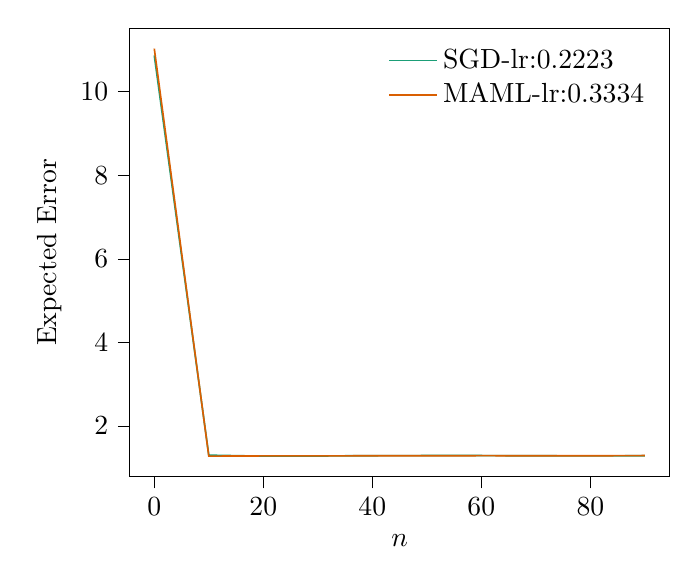
\begin{tikzpicture}

\definecolor{color0}{rgb}{0.105882352941176,0.619607843137255,0.466666666666667}
\definecolor{color1}{rgb}{0.850980392156863,0.372549019607843,0.00784313725490196}

\begin{axis}[
legend cell align={left},
legend style={fill opacity=0.8, draw opacity=1, text opacity=1, draw=none},
tick align=outside,
tick pos=left,
x grid style={white!69.0196078431373!black},
xlabel={\(\displaystyle n\)},
xmin=-4.5, xmax=94.5,
xtick style={color=black},
y grid style={white!69.0196078431373!black},
ylabel={Expected Error},
ymin=0.791511754079209, ymax=11.515920737703,
ytick style={color=black}
]
\addplot [semithick, color0]
table {%
0 10.8643227049792
10 1.30264702485407
20 1.27898488969847
30 1.28358354249911
40 1.29062835599866
50 1.29336012947113
60 1.29313886133164
70 1.28811089224953
80 1.28544374192371
90 1.28803444049909
};
\addlegendentry{SGD-lr:0.2223}
\addplot [semithick, color1]
table {%
0 11.0284476020837
10 1.27973217276018
20 1.28540821831848
30 1.28531771660341
40 1.28806432300703
50 1.28812612553632
60 1.29123331123801
70 1.2900164318019
80 1.28917008656963
90 1.29331539237872
};
\addlegendentry{MAML-lr:0.3334}
\end{axis}

\end{tikzpicture}
